\paragraph{lakeFS}
\cite{lakefs}
Similarly to DVC, LakeFS is a format-agnostic solution. Similarly to Git LFS and
DVC, it works on basis of file pointers being stored in a Key Value Store (such
as Postgres Database) and the content of the files being stored in Object Store
Bucket (support of S3 compatible systems) (Figure
\ref{fig:dvc-architecture})\cite{architecture-lakefs}. While lacking in certain
features of DVC (data pipelines definitions and visualisations), it offers
higher degree of scalability by implementation of immutable ranges. Range is a
set of pointers to files (in sorted order), containing metadata. Metaranges
contain ranges, with commit serving as a pointer to a set of metaranges. Thus,
when modifying files we can reuse certain ranges, that have not been modified,
which leads to more efficient storage management (Figure
\ref{fig:lakefs-ranges}). 

\begin{figure}[H]
    \centering
    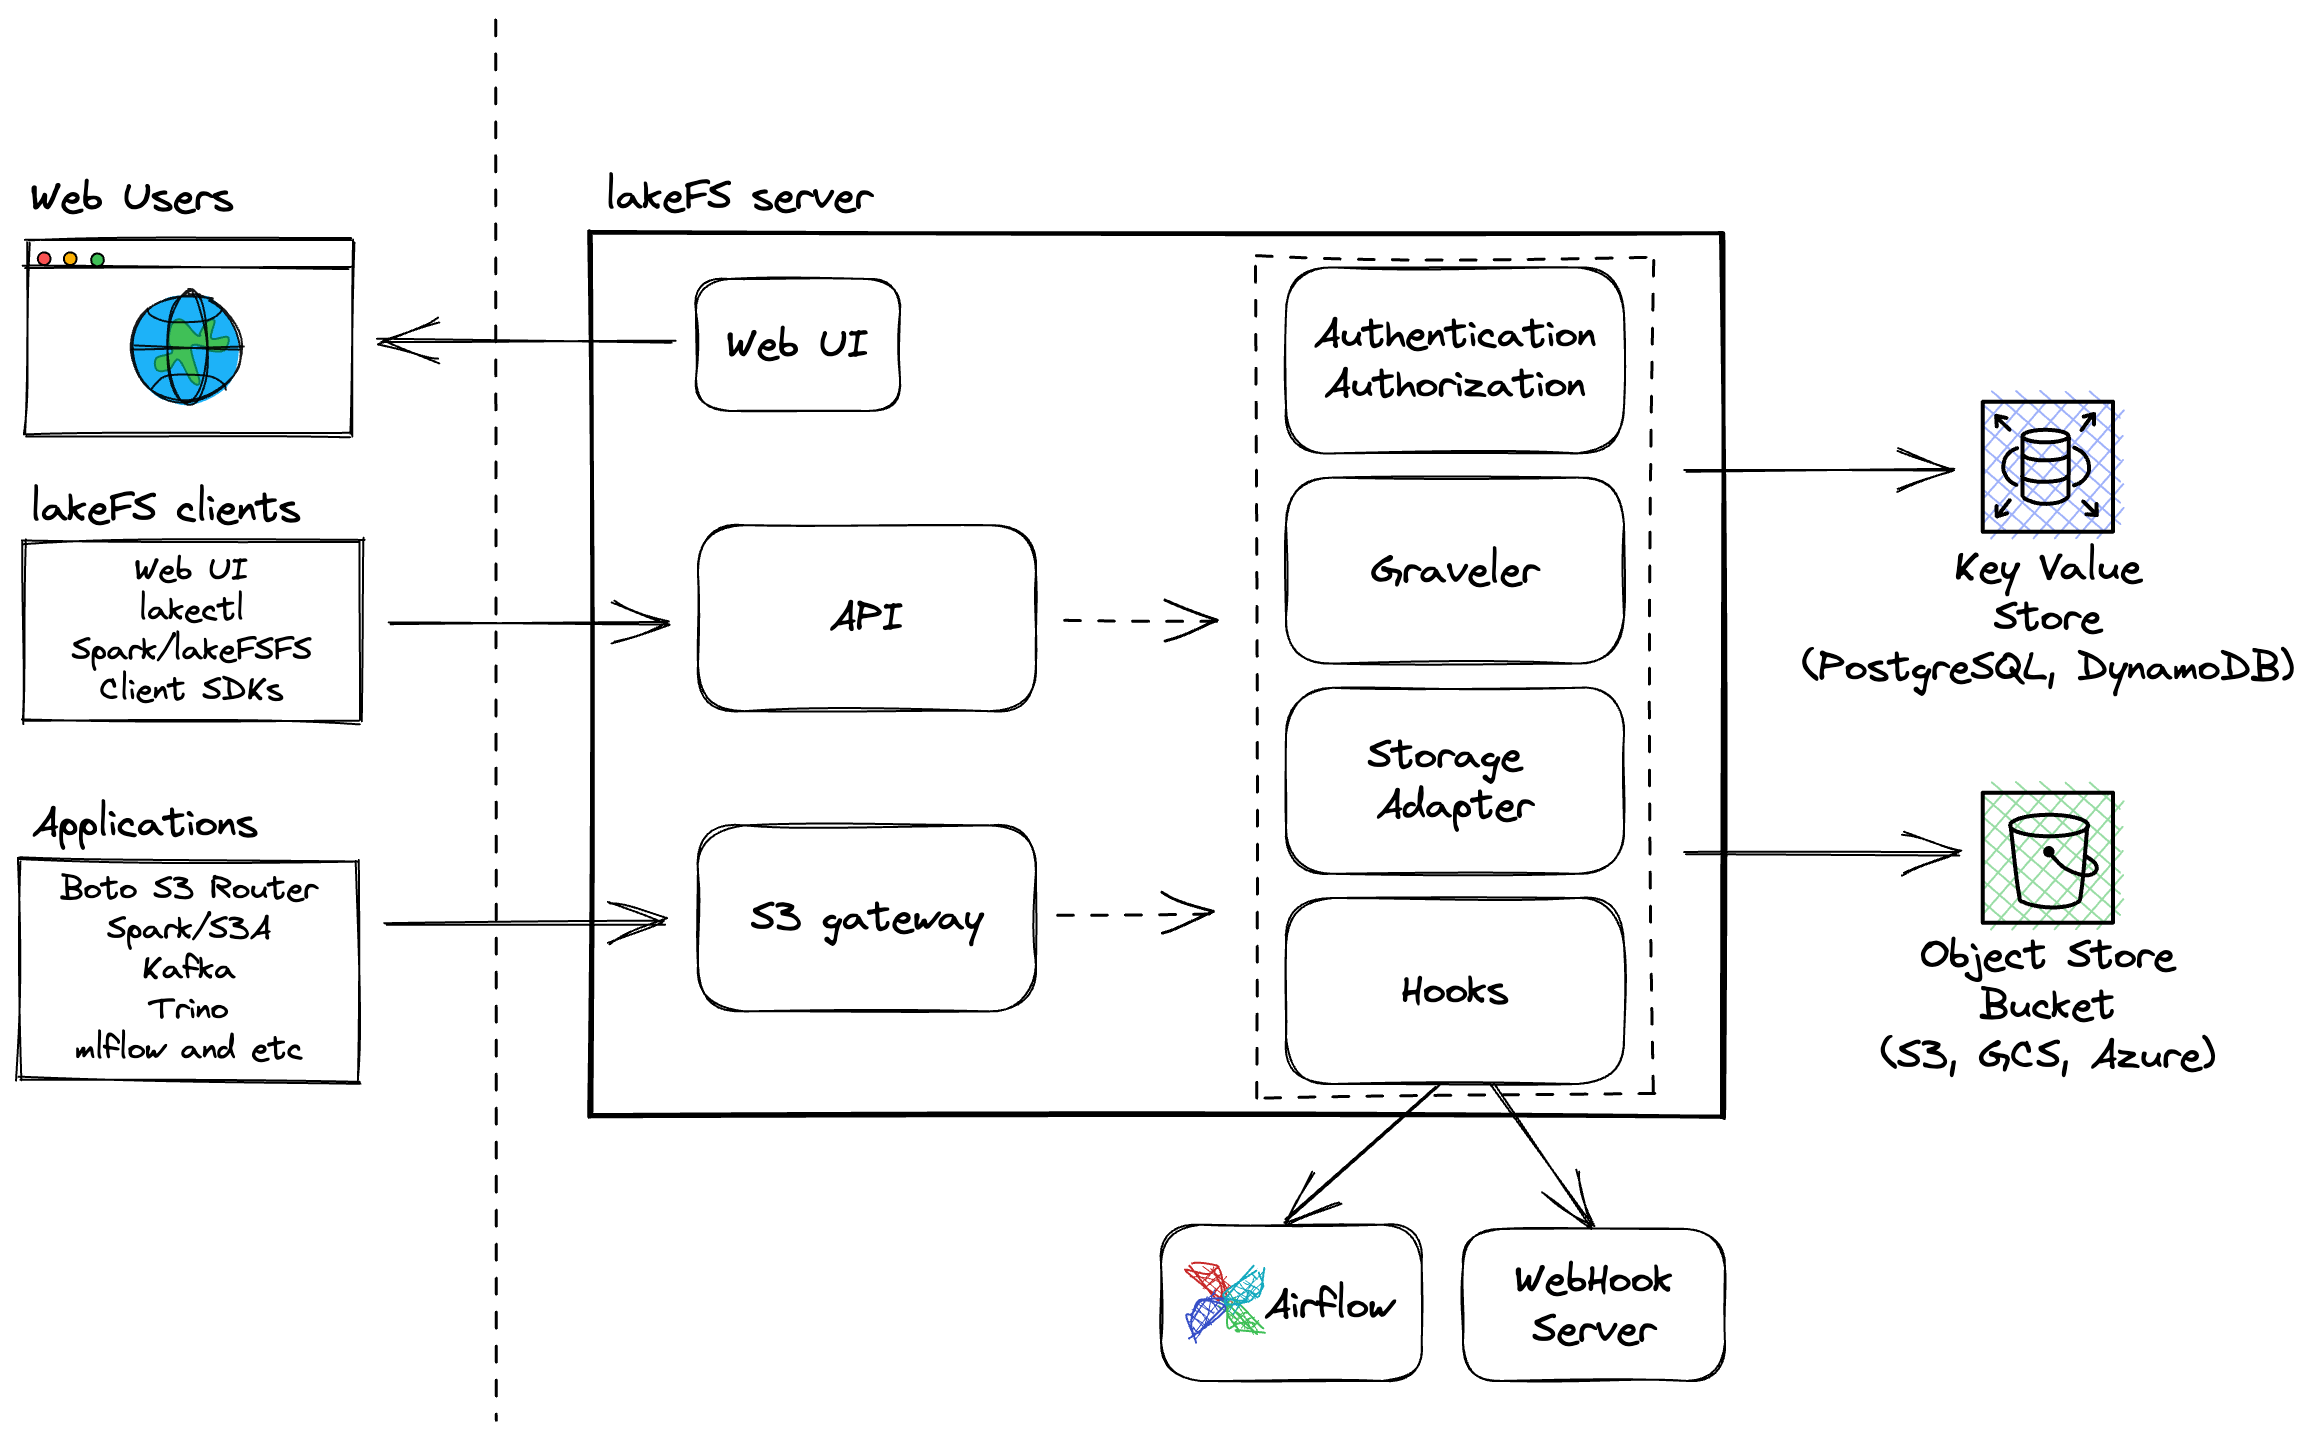
\includegraphics[width=0.8\textwidth]{fig/lakefs-arch.png}
    \caption{Software architecture of LakeFS \cite{architecture-lakefs}}
    \label{fig:lakefs-architecture}
\end{figure}

\begin{figure}[H]
    \centering
    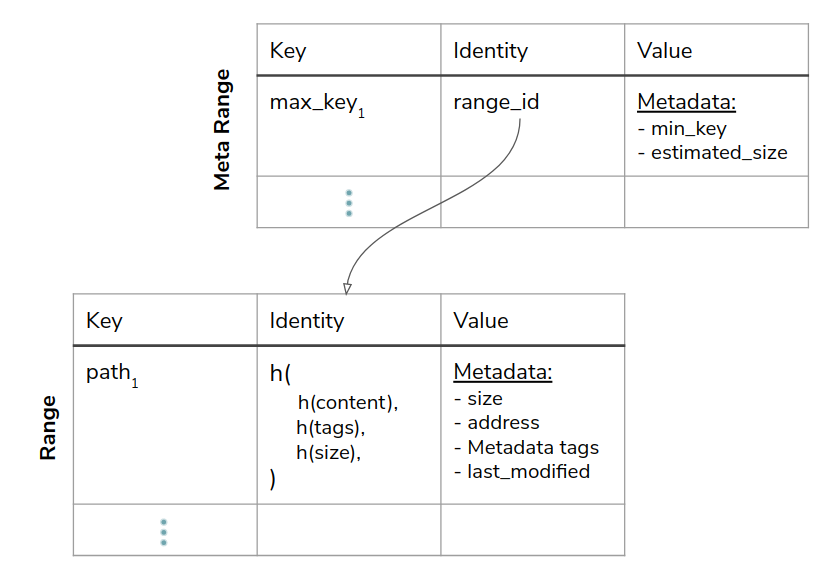
\includegraphics[width=0.8\textwidth]{fig/graveler2.png}
    \caption{Diagram showcasing ranges \cite{architecture-lakefs}}
    \label{fig:lakefs-ranges}
\end{figure}

\begin{comment}
zero-copy branching - no data duplication
configurable garbage collection
format-agnostic (both structured and unstructed)
data management using S3 interface (AWS S3, Google Cloud Storage, Azure Blob Storage)
uses metafiles (similar to DVC)
tools for CI/CD
can be ran locally or in cloud

https://stackoverflow.com/questions/846659/how-can-i-put-a-database-under-git-version-control
https://www.youtube.com/watch?v=1vNQXFceFx4&t=14s
https://medium.com/datamindedbe/what-is-lakefs-a-critical-survey-edce708a9b8e

maybe something more about datalakes?
spomen caching (respektive jeho neexistenciu)
\end{comment}